\documentclass{article}
\usepackage[numbers,sort&compress]{natbib}
\usepackage{graphicx}
\usepackage{amssymb,amsmath}
\usepackage{bm}
\usepackage{color}
\usepackage{tabularx}

\newcommand{\beq}{\begin{equation}}
\newcommand{\feq}{\end{equation}}
\newcommand{\beqstar}{\begin{equation*}}
\newcommand{\feqstar}{\end{equation*}}                                     
\newcommand{\beqal}{\begin{equation}\begin{aligned}}
\newcommand{\feqal}{\end{aligned}\end{equation}}
\newcommand{\beqalstar}{\begin{equation*}\begin{aligned}}
\newcommand{\feqalstar}{\end{aligned}\end{equation*}}
\newcommand{\vol}{k_L\,a}

\begin{document}
\section{Motivation}
The mass transfer is a very important characteristic for microchannels  design. It allows to
properly manufacture a microchannel with necessary properties to ensure that chemical
reactions are performed in the best manner. In
what follows the mass transfer associated with the bubble moving in the microchannel through liquid
medium is studied. 

A few questions need to be addressed:
\begin{description}
 \item[I] The efficiency of the mass transfer depending on the capillary number. For small capillary
numbers as $Ca<0.6$ for square microchannels there is a vortex in the reference frame moving with
the bubble, which  influences and improves the corresponding mass transfer. 
Note that the flow
patterns strongly depend on the number of parameters as the slug length, the thickness of the
thickness and the existence of the vortex in front of the bubble. There are some available
correlations in literature \cite{bercic-mass,kreutzer-overview} and one of the particular goal of
this work is to study mass transfer dependence on the number of parameters. Another goal is to
validate and to come up with another correlation describing the mass transfer.

 \item[II] Another important quantity is to study the mixing processes inside the slug. One of the
possible characteristics of the mixing is a residence time distribution. Once the step function
of tracer is introduced in the liquid film, then the concentration of tracer with time is
measured at the outlet. The form of the signal and especially its standard deviation is responsible
for mixing. However, from numerical point of view this study requires the repetition of domain a
few times to see the tracer propagation. Thus, we do not currently address mixing with our
simulations.
\end{description}

To address the questions arised we will utilize the results of numerical simulations of flow
obtained
before \cite{kuzmin-binary2d}. The numerical benchmark is presented in Fig. \ref{fig:benchmark}. In
the same figure, one can see the proposed benchmark for the tracer. The
physical
picture for the proposed numerical benchmark is  related to classical experiments conducted by
\citet{bercic-mass}. In their work authors studied gas-liquid mass transfer coefficient by
injecting methane as the gas bubble and measuring the dissolved concentration of methane in water
along the channel. This situation implies the periodic boundary conditions and steady-state motion
of bubbles.  

The numerical  procedure of studying mass transfer is presented in the following steps:
\begin{description}
 \item[Flow field] The hydrodynamics for the bubble motion in the periodic domain is obtained
according to the work \cite{kuzmin-binary2d}. The grid resolution is taken to insure grid
independency of results.  
 \item[Bubble reference frame] Once the hydrodynamics is resolved, the mass transfer simulations
are conducted in the moving
reference frame with the bubble. Then the bubble stands still and the flow is coming around the
bubble. We impose a steady concentration of solutant on the surface of the bubble.
\item[Mass transfer] One needs not only perform a Galilean transformation to the reference
frame moving with the bubble but also to
transfer the bubble to the inlet condition. This can insure that the studied phenomenon is a liquid
slug. 
\end{description}
\begin{figure}[htb!]
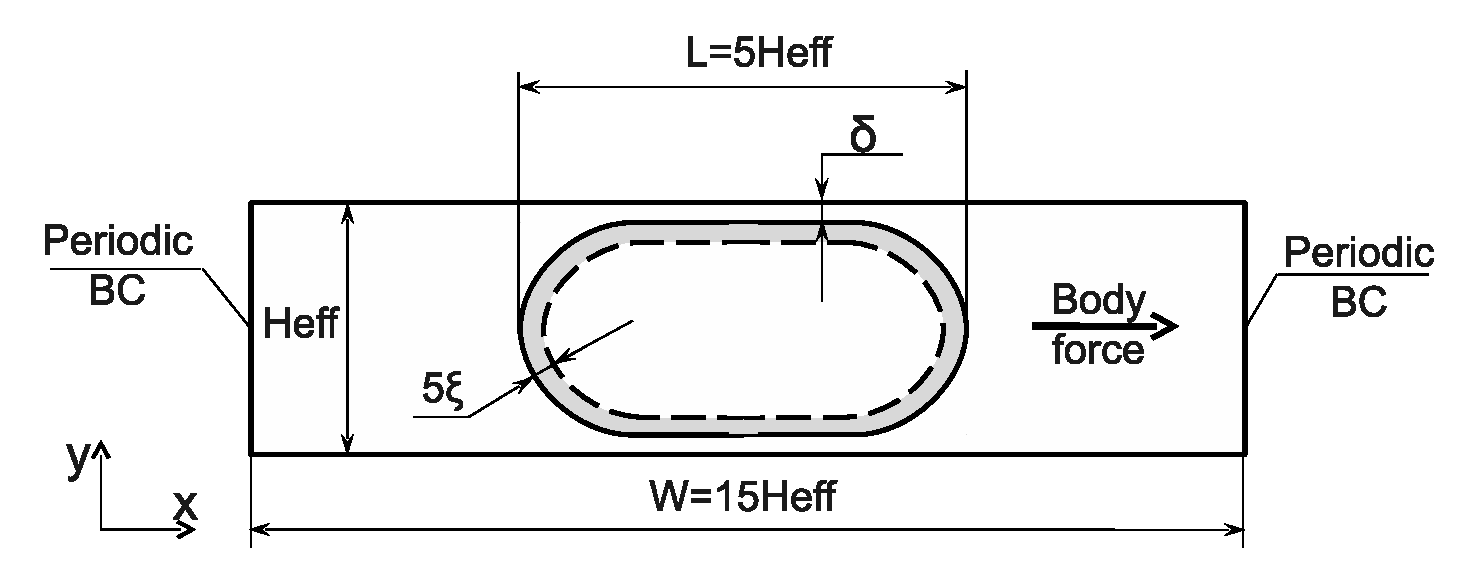
\includegraphics[width=\textwidth]{Figures/benchmark_new.eps}\\
\\
\\
\\
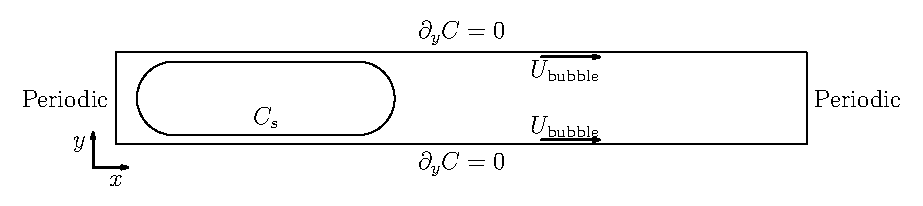
\includegraphics[width=\textwidth]{Figures/benchmark_periodic.eps}
\caption{The two-dimensional benchmarks for the hydrodynamics (top) and the mass transfer
coefficient (bottom). \label{fig:benchmark}}
\end{figure}

\section{Mass Transfer Correlations}
\label{sec:correlations}
We examine the following three characteristic correlations:
\begin{description}
\item[I]
In what follows we want to address the following empirical correlation for the volumetric mass
transfer coefficient addressed in the recent
publication by \citet{yue-mass}:
\begin{equation}
k_L a=\frac{2}{d_h} \Bigl(\frac{D
U_{\mathrm{bubble}}}{L_{\mathrm{bubble}}+L_{\mathrm{slug}}}\Bigr)^{0.5}
\Bigl(\frac{L_{\mathrm{bubble}}}{L_{\mathrm{bubble}}+L_{\mathrm{slug}}}\Bigr)^{0.3}.
\end{equation}
This correlation is within $10\%$ accuracy for experimental results for the following range of
parameters: bubble velocity $0.4\,\mathrm{m/s}<U_{\mathrm{bubble}}<2\,\mathrm{m/s}$, bubble length
$1.4<\frac{L_{\mathrm{bubble}}}{d_h}<6.3$, slug length $1<\frac{L_{\mathrm{slug}}}{d_h}<3.2$,
hydrodynamic diameter $d_h = 400
\mathrm{\mu m}$.

\item[II]
For long slug lengths in circular capillaries, where the mass transfer from bubble caps is
predominant, the folowing correlation is derived by
\citet{bercic-mass}:
\begin{equation}
k_L a = \frac{0.111
(U_{\mathrm{gas}}+U_{\mathrm{liq}})^{1.19}}{\bigl((1-\varepsilon_{\mathrm{gas}})(L_{\mathrm{bubble}}
+L_ {\mathrm{slug}} )\bigr)^{0.57} },
\end{equation}
where $\varepsilon_{\mathrm{gas}}=\frac{U_{\mathrm{gas}}}{U_{\mathrm{bubble}}}$ is the gas holdup,
$U_{\mathrm{gas}}$ is the superficial gas velocity, and $U_{\mathrm{liq}}$ is the superficial
liquid velocity. The superficial liquid velocity is calculated with the steady state condition in
the middle of the slug as:
\begin{equation}
U_{\mathrm{liq}}=\frac{\oint U \mathrm{d}A}{A}.
\end{equation}
The superficial liquid velocity can be calculated through the calculated bubble volume and gas
holdup. For the two-dimensional case it is represented as:
\begin{equation}
\begin{aligned}
&\varepsilon_{\mathrm{gas}}=\frac{\text{bubble area}}{15 H^2}\\
&U_{\mathrm{gas}}=\varepsilon_{\mathrm{gas}} U_{\mathrm{bubble}}.
\end{aligned}
\end{equation}

Since experiments done by \citeauthor{bercic-mass} were only for one diffusivity coefficient
$D=2\times 10^{-9}\,\mathrm{m^2/s}$, the effective equation should be rescaled as:
\begin{equation}
k_L a = \sqrt{\frac{D}{2\times 10^{-9}\,\mathrm{m^2/s}}}\frac{0.111
(U_{\mathrm{gas}}+U_{\mathrm{liq}})^{1.19}}{\bigl((1-\varepsilon_{\mathrm{gas}})(L_{\mathrm{bubble}}
+L_ {\mathrm{slug}} )\bigr)^{0.57} },
\end{equation}

\item[III]
\citet{vanbaten-circular} performed numerical simulations for circular capillaries by assuming that
there is a separate contribution of the liquid film and the bubble caps to mass transfer. Their
correlation is as:
\begin{equation}
k_L a = \frac{2}{\sqrt{\pi}}\sqrt{\frac{D U_{\mathrm{bubble}}}{(L_{\mathrm{bubble}}-d_h)}}
\frac{4(L_{\mathrm{bubble}}-d_h)}{d_h(L_{\mathrm{bubble}}+L_{\mathrm{slug}})}+2\frac{\sqrt{2}}{\pi}
 \sqrt{\frac{D U_{\mathrm{bubble}}}{d_h}} \frac{4}{(L_{\mathrm{bubble}}+L_{\mathrm{slug}})}.
\end{equation}
This correlation is valid for short contact times, when the mass transfer is important from bubble
caps as well as from the film. Short contact times are defined through Fourier number as:
\begin{equation}
Fo=\frac{D t_{\mathrm{film}}}{\delta^2},
\end{equation}
where $t_{\mathrm{film}}=\frac{L_{\mathrm{film}}}{U_{\mathrm{bubble}}}$ is the time exposure of the
bubble while it propagates through distance $L_{\mathrm{film}}$. The Fourier number is assumed to
be small if $Fo<0.1$. If $Fo>1$ then the liquid film is saturated and the mass transfer occurs from
the bubble caps.

\end{description}

Overall work goal is to compare numerical simulations with given correlations and to establish a
new one.

\section{Mass transfer}
The mass transfer is characterized by non-dimensional numbers as Schmidt number (viscous diffusion
rate over mass diffusion rate), the Peclet number (convection over diffusion) and the Sherwood
number (convection mass transfer over diffusion mass transfer):
\begin{equation}
\begin{aligned}
&Pe=\frac{U L}{D}\\
&Sh=\frac{K L}{D}\\
&Sc=\frac{\nu}{D}\\
\end{aligned}
\end{equation}

As far as the lattice Boltzmann method operates only in the non-dimensional space, one needs to
match the non-dimensional lattice Boltzmann parameters with non-dimensional physical parameters.
Therefore, one needs to form non-dimensional numbers from the physical parameters. One of the
particular experiment examples is the
work by \citet{bercic-mass} who used the methane dissolution to characterize the mass transfer for
bubble train flow. 

In what follows we will perform the matching of obtained hydrodynamics results
\cite{kuzmin-binary2d} with physical ones from experiment of \citet{bercic-mass}. The diffusion
coefficient of the methane under standard conditions \cite{methane-properties} is
$1.84\times 10^{-5} \mathrm{cm}^2/\mathrm{s}$. The diameters of capillaries in the experiment were
as $1.5$, $2.5$ and
$3.1\,\mathrm{mm}$. For simplicity reasons we will choose the diameter of capillary as $1.5\,
\mathrm{mm}$. 
The non-dimensional parameters obtained from the hydrodynamics lattice Boltzmann simulations are
as:
\begin{equation}
\begin{aligned}
&Ca=\frac{U \mu_{\mathrm{liq}}}{\gamma}\\
&Re=\frac{\rho_{\mathrm{liq}} U L}{\mu_{\mathrm{liq}}}.
\end{aligned}
\end{equation}
Given some physical characteristics as the liquid density and the channel length,
one can obtain the physical velocity obtained from non-dimensional numbers:
\begin{equation}
\begin{aligned}
Ca\cdot Re= \frac{\rho_{\mathrm{liq}} U^2 L}{\gamma}\\
U=\sqrt{\frac{Ca\,Re\,\gamma}{\rho_{\mathrm{liq}}L}}
\end{aligned}
\end{equation}

Assuming that the surface tension of water is $0.0728\,\mathrm{N/m}$ (methane exhibits the same
trend \cite{schmidt-methane}), the density is       
$1000\,\mathrm{kg/m^3}$, the hydraulic diameter of the channel to be $1.5\,\mathrm{mm}$ one can
calculate the physical velocity of the bubble.
Table \ref{table:twod:simulations} represents lattice Boltzmann simulations results and their
physical equivalents for the grid $202\times 3002$. One can see
that velocity is quite reasonable
as \citet{bercic-mass} declared that experiments were conducted for velocities in the ranges of
$0.01$ to $0.4\,\mathrm{m}/\mathrm{s}$. 
\begin{table}
\begin{tabularx}{\textwidth}{|X|X|X|X|X|X|}
\hline
$Ca$    &$Re$     &$U_{LB}$ &$\delta$&$\varepsilon_{\mathrm{gas}}$
&$U_{\mathrm{phys}}, \mathrm{m/s}$\\
\hline
$0.026$ &$0.449$  &$0.0014$ &$0.040$ &$0.306$ &$0.023$   \\ 
$0.047$ &$0.820$  &$0.0027$ &$0.058$ &$0.293$ &$0.043$   \\ 
$0.080$ &$1.378$  &$0.0045$ &$0.085$ &$0.280$ &$0.073$ \\
$0.065$ &$1.126$  &$0.0037$ &$0.076$ &$0.266$ &$0.059$      \\
$0.222$ &$3.807$  &$0.0125$ &$0.122$ &$0.253$ &$0.202$  \\
$0.479$ &$8.222$  &$0.0271$ &$0.151$ &$0.249$ &$0.437$  \\
$0.736$ &$12.617$ &$0.0416$ &$0.164$ &$0.236$ &$0.671$  \\ 
$0.989$ &$16.960$ &$0.0559$ &$0.172$ &$0.230$ &$0.902$  \\
\hline
\end{tabularx}
\caption{Two-dimensional simulations for different
capillary numbers. \label{table:twod:simulations}}
\end{table}

\section{Lattice Boltzmann implementation}
For the lattice Boltzmann implementation we took $\omega=1.99$ which results in the following
lattice Boltzmann diffusivity parameter:
\begin{equation}
\begin{aligned}
&D=\frac{1}{3}\Bigl(\frac{1}{\omega}-\frac{1}{2}\Bigr)\\
&D=0.0008375
\end{aligned}
\end{equation}
In terms of the Schmidt number (taking the lattice Boltzmann liquid viscosity in former simulations
as $\frac{2}{3}$) that
can result in:
\begin{equation}
\begin{aligned}
&Sc=\frac{\nu_{\mathrm{liq}}}{D}\\
&Sc=796\\
\end{aligned}
\end{equation}
Taking the water dynamic viscosity as $8.9 \times 10^{-4}\,\mathrm{Pa\cdot s}$ or kinematic
viscosity as $8.9 \times
10^{-7} \,\mathrm{m^2/s}$ and the Schmidt number as $796$ results in the following physical
diffusion coefficient:
\begin{equation}
D=1.118\times 10^{-5}\,\mathrm{cm^2/s},
\end{equation}
which is less than the diffusivity of the methane $1.84\times 10^{-5}\,\mathrm{cm^2/s}$ but is
physical. After calculation of physical parameters one can calculate correlations indicated in
Section \ref{sec:correlations} for mass transfer. Table \ref{table:lengths} presents extraction
from the lattice Boltzmann simulation necessary to calculate mass transfer calculations.
For the two-dimensional case parameter  $a$ is defined as:
\begin{equation}
a = \frac{\text{bubble perimeter}}{\text{cell area}}.
\end{equation}
For the height of the channel to be $H=1.5 \times 10^{-3}\,\mathrm{m}$, parameters $a$ are
presented in Table \ref{table:lengths}. 
\begin{table}
\begin{tabularx}{\textwidth}{|X|X|X|X|X|X|}
\hline
$Ca$&Bubble length& Slug Length&
$U_{\mathrm{gas}},\,\mathrm{m/s}$&$U_{\mathrm{liq}},\,\mathrm{m/s}$&$a,\,\mathrm{m^{-1}}$\\
\hline
$0.026$&$5.225$&$9.775$ &$0.0070$ &$0.0209$&$510.77$\\
$0.047$&$5.22$ &$9.78$  &$0.0126$ &$0.0379$&$508.62$\\
$0.080$&$5.215$&$9.785$ &$0.0204$ &$0.0615$&$506.53$\\
$0.065$&$4.965$&$10.035$&$0.0157$ &$0.0504$&$482.84$\\
$0.222$&$5.25$ &$9.75$  &$0.0511$ &$0.1560$&$505.06$\\
$0.479$&$5.565$&$9.435$ &$0.1089$ &$0.3155$&$530.37$\\
$0.736$&$5.51$ &$9.49$  &$0.1584$ &$0.4677$&$525.38$\\
$0.989$&$5.505$&$9.495$ &$0.2074$ &$0.6190$&$526.80$\\
\hline
\end{tabularx}
\caption{The nondimensional (scaled to the height of the channel) lengths for the same
lattice Boltzmann simulations as in Table \ref{table:twod:simulations}. As well superficial
gas and liquid velocities are presented. \label{table:lengths}} 
\end{table}

The literature correlations of mass transfer dependence on the bubble velocities are presented in
Fig. \ref{fig:mass:transfer:theoretical}. Note, that the correlations presented in
Fig. \ref{fig:mass:transfer:theoretical} are used primarily for circular capillaries
(\citeauthor{vanbaten-circular,bercic-mass}) and for square capillaries (\citeauthor{yue-mass}). We
adapt these results for flow between parallel plates by using hydraulic
diameter \cite{bercic-mass} which can be calculated as:
\begin{equation}
d_h = \lim_{W\to\infty}\frac{4A}{P}=\lim_{W\to\infty}\frac{4 W\,H}{2(W+H)}=2 H.
\end{equation}
For comparison reasons we derived in Section \ref{mass:transfer:correlation} the correlation for the
flow between plates, see Fig. \ref{fig:mass:transfer:theoretical}. One can see that the
difference is negligible.

\begin{figure}[htb!]
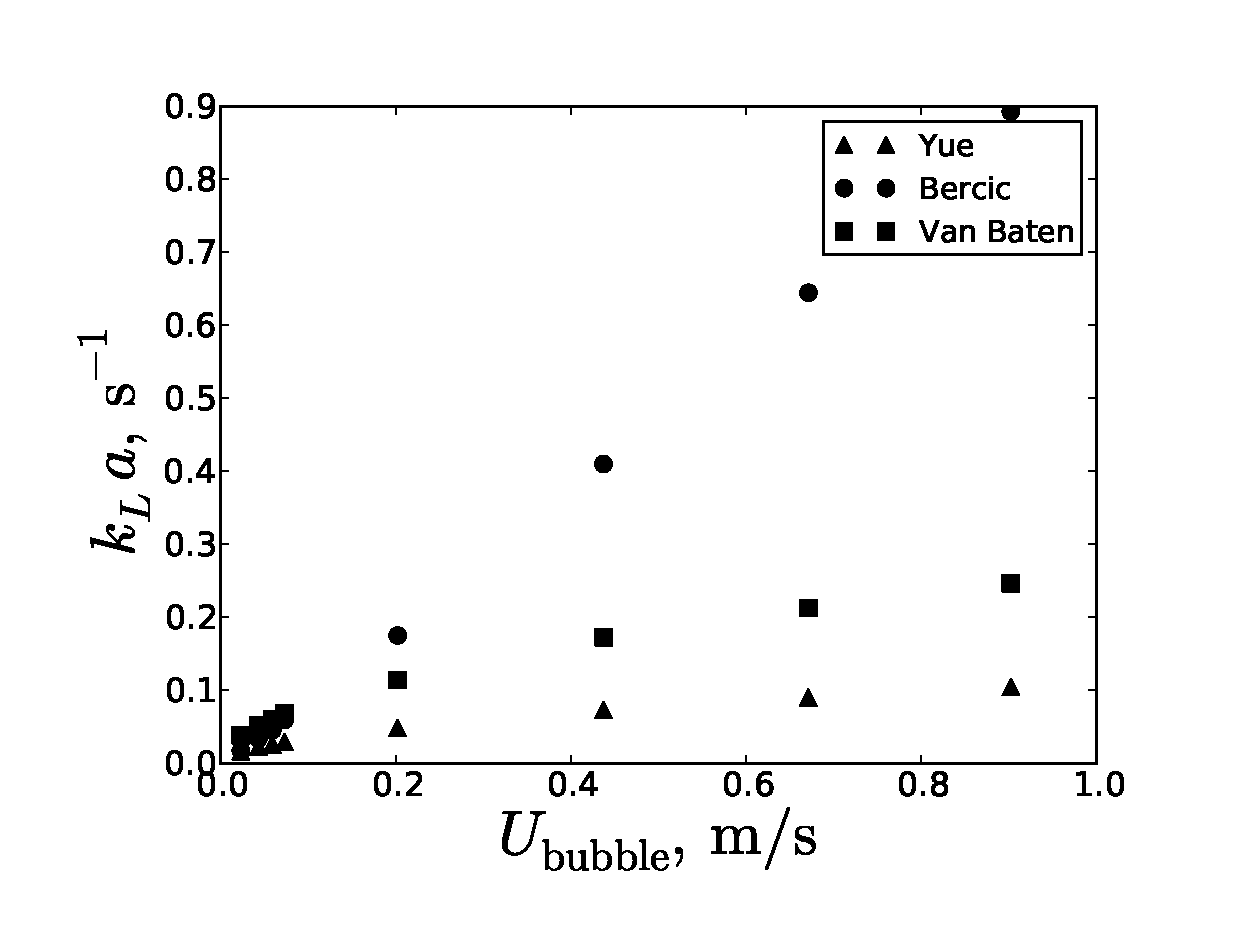
\includegraphics[width=\textwidth]{Figures/theoretical_correlations.eps}\\
%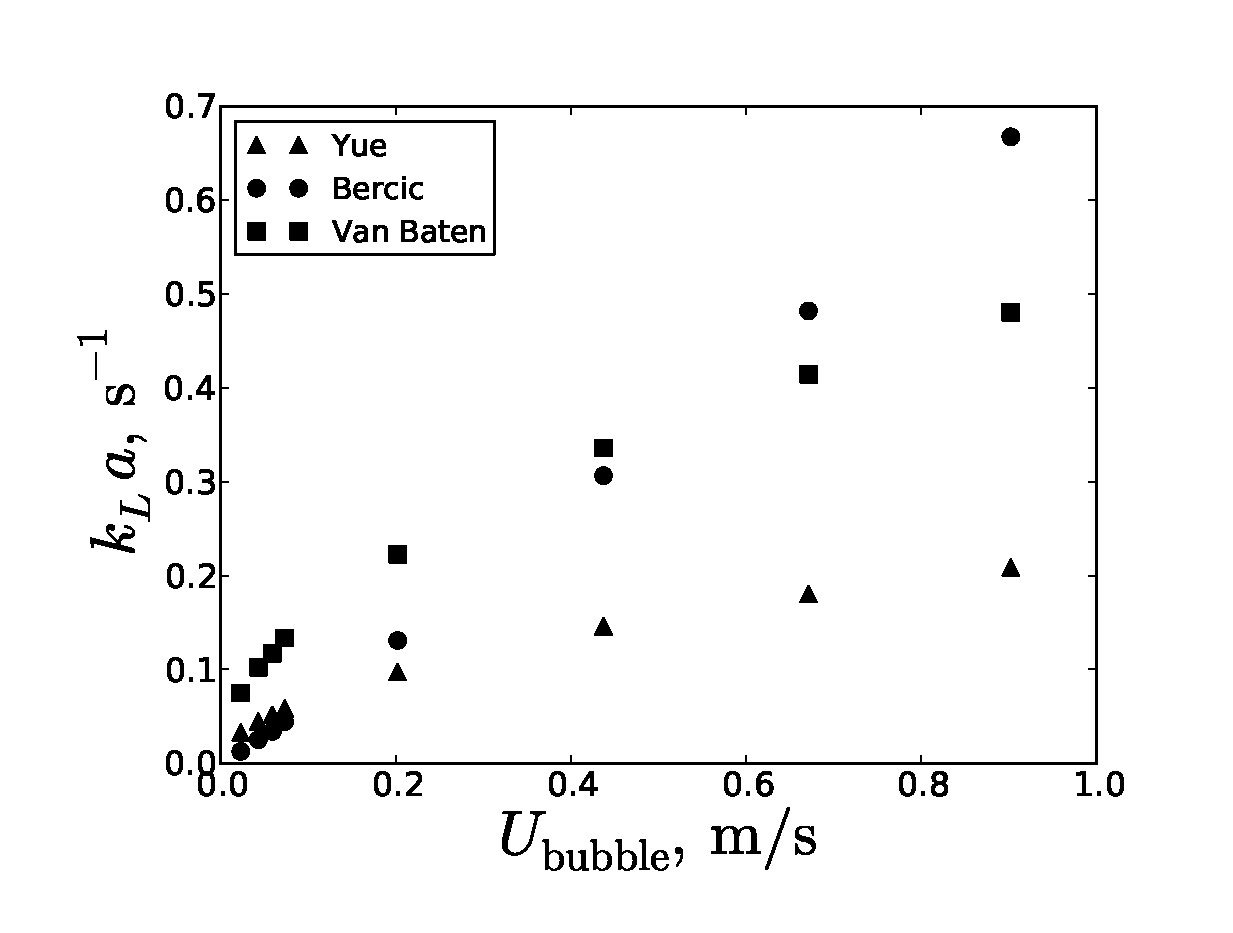
\includegraphics[width=\textwidth]{Figures/theoretical_correlations_without_hydraulic.eps}\\
\caption{The literature correlations by various authors.\label{fig:mass:transfer:theoretical}}
\end{figure}

The volumetric mass transfer coefficient is calculated according to the work of
\citet{vanbaten-circular}. The concentration flux is calculated as the difference between overall
average concentration taken in the whole domain ($C_{overall}=\int_{V} C \mathrm{d}V /V$)
at time
$t_1$ and time $t_2$ divided on the time difference $t_2-t_1$ {\color{red} (In this particular
moment I don't know whether to take the volume of the whole domain or
just the liquid phase. I will go for whole domain.)}. Then the volumetric mass transfer
coefficient is calculated as \cite{vanbaten-circular}:
\begin{equation}
\label{main:simulation:equation}
k_L a=\frac{\text{Flux}}{C_s-C_{outlet}} \frac{\text{bubble surface area}}{\text{unit cell volume}},
\end{equation}
where $C_{outlet}=\int{C U_{outlet}\mathrm{d}A}/\int{U_{outlet}\mathrm{d}A}$. 
{\color{red} Do not understand why we need this ratio bubble surface area/unit cell volume. In this
case the dimensional units do not coincide. In the calculations I will avoid it until further
clearance.} The overall concentration in the lattice Boltzmann system is prescribed as:
\begin{equation}
C_{overall}=\frac{\sum{c_i}}{N_x \, (N_y-2)}.
\end{equation}

To properly do
non-dimensioanalization one needs to insure the time conversion factor when the flux is calculated
inside the lattice Botlzmann system. The time conversion can be easily obtained:
\begin{equation}
\begin{aligned}
&U_{LB}=U_{phys}\frac{\Delta t}{\Delta x}\\
&\Delta t=\frac{U_{LB}}{U_{phys}}\Delta x\\
&\Delta t=\frac{1.5\,\mathrm{mm}}{200} \frac{0.0559}{0.902\,\mathrm{m/s}}=4.64\times
10^{-7}\,\mathrm{s} 
\end{aligned}
\end{equation}

The bubble surface length is the perimeter of the bubble in two-dimensional space and it is
calculated with the extraction of the bubble contour and representing it with the polygon. After
that the calculated perimeter is the effective summation of line lengths and can be represented as:
\begin{equation}
P=\sum_i{\sqrt{(x2_i-x1_i)^2+(y2_i-y1_i)^2}},
\end{equation}
where the index $i$ represents the polyline consisting of two points $(x1,y1)$ and $(x2,y2)$.
%The corresponding volumetric mass transfer coefficients depending on the velocity are indicated in
%Table \ref{table:volumetric:coefficients}.

\section{Simulation results}
\subsection{Steady-state}
Using Eq.\ref{main:simulation:equation} we calculated the mass transfer coefficient. One can see
the plots for the mass transfer coefficient versus time in Fig. \ref{fig:steady:state}. We state as
a steady-state condition the average of concentration values between $500000$ to $1000000$ time
steps.{\color{red} We need to put more time steps. As well it is probably connected with Fourier
number.} The average calculated volumetric mass transfer coefficients values are presented in Table
\ref{table:volumetric:coefficients}. For each of the measurements we as well provided the Fourier
number (for the flow between plates is as follows):
\begin{equation}
Fo=\frac{D t_{\mathrm{film}}}{\delta^2}=\frac{D
(L_{\mathrm{bubble}}-H)}{U_{\mathrm{bubble}}\delta^2}.
\end{equation}
To understand the influence of the mass transfer in the film we provided the time needed for
diffusion to reach the film thickness distance (95\% confidence interval of the film thickness):
\begin{equation}
\delta\approx 2\sqrt{2}\sqrt{D t};\ t \approx \frac{\delta^2}{8 D};\ N_{iter}=\frac{t}{\Delta t}.
\end{equation}

\begin{figure}[htb!]
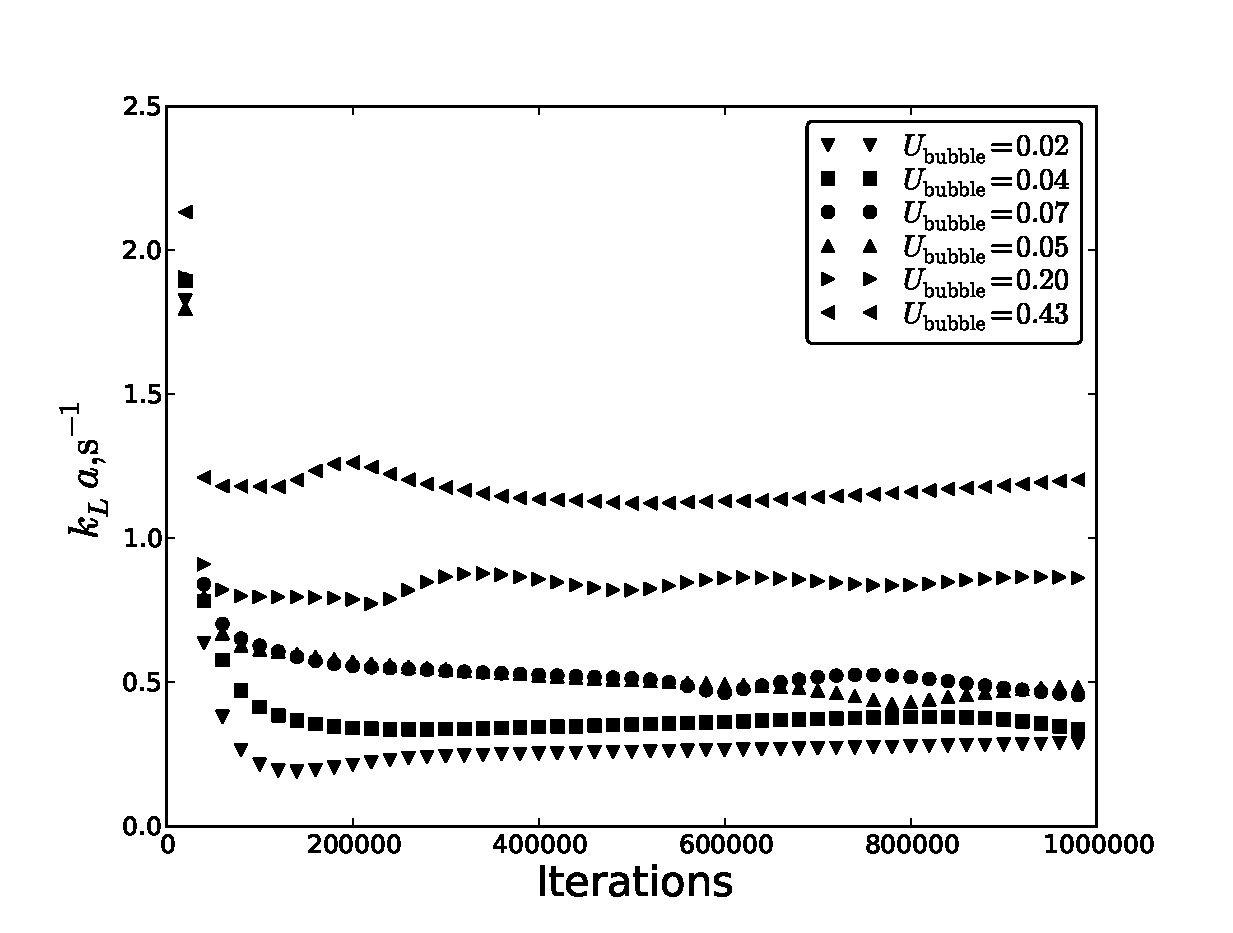
\includegraphics[width=\textwidth]{Figures/steady_state.eps}
\caption{The mass transfer coefficient vs. time iterations. One can see that the pseudo steady
state can be reached after $500000$. The mass transfer coefficient is taken as the average of
concentration values between $500000$ to $1000000$ time steps.\label{fig:steady:state}}
\end{figure}
\begin{table}[htb!]
\begin{tabularx}{\textwidth}{|X|X|X|X|}
\hline
$Ca$&$Fo$&$k_L a,\,\mathrm{s}^{-1}$&$N_{iter}$\\
\hline
$0.026$&$0.08493$&$0.2737$&$873984$\\
$0.047$&$0.02160$&$0.3664$&$1835817$\\
$0.080$&$0.00588$&$0.4959$&$3965227$\\
$0.065$&$0.00862$&$0.4734$&$3149710$\\
$0.222$&$0.00103$&$0.8505$&$8195770$\\
$0.479$&$0.00034$&$1.1541$&$12399627$\\
$0.736$&$0.00018$&$1.1801$&$14683652$\\
$0.989$&$0.00012$&$1.2215$&$16101062$\\
\hline
\end{tabularx}
\caption{Simulation results for different capillary numbers. \label{table:volumetric:coefficients}}
\end{table}

\subsection{Comparison between different boundary conditions}
The mass transfer coefficient by the definition of used in the paper of \citet{vanbaten} is as
follows:
\begin{equation}
dd
\end{equation}


In what follows we will examine different boundary conditions for the mass transfer:
\begin{description}
 \item[I] Placement the bubble near the entrance with the periodic bondary conditions and using the
outlet concentration as the characteristic value of the 
\item[II] 
\end{description}

\begin{figure}[htb!]
\caption{Comparison between different simulations and definitions of the characteristic
concentration.}
\end{figure}


\subsection{Comparison between correlations and results}
Comparison between correlations and simulations one can find in Fig.
\ref{fig:comparison:correlations}. The simulated results exhibit larger mass transfer in comparison
with the given correlations. {\color{red} Need to recalculate and check the kinematic viscosities.}
\begin{figure}[htb!]
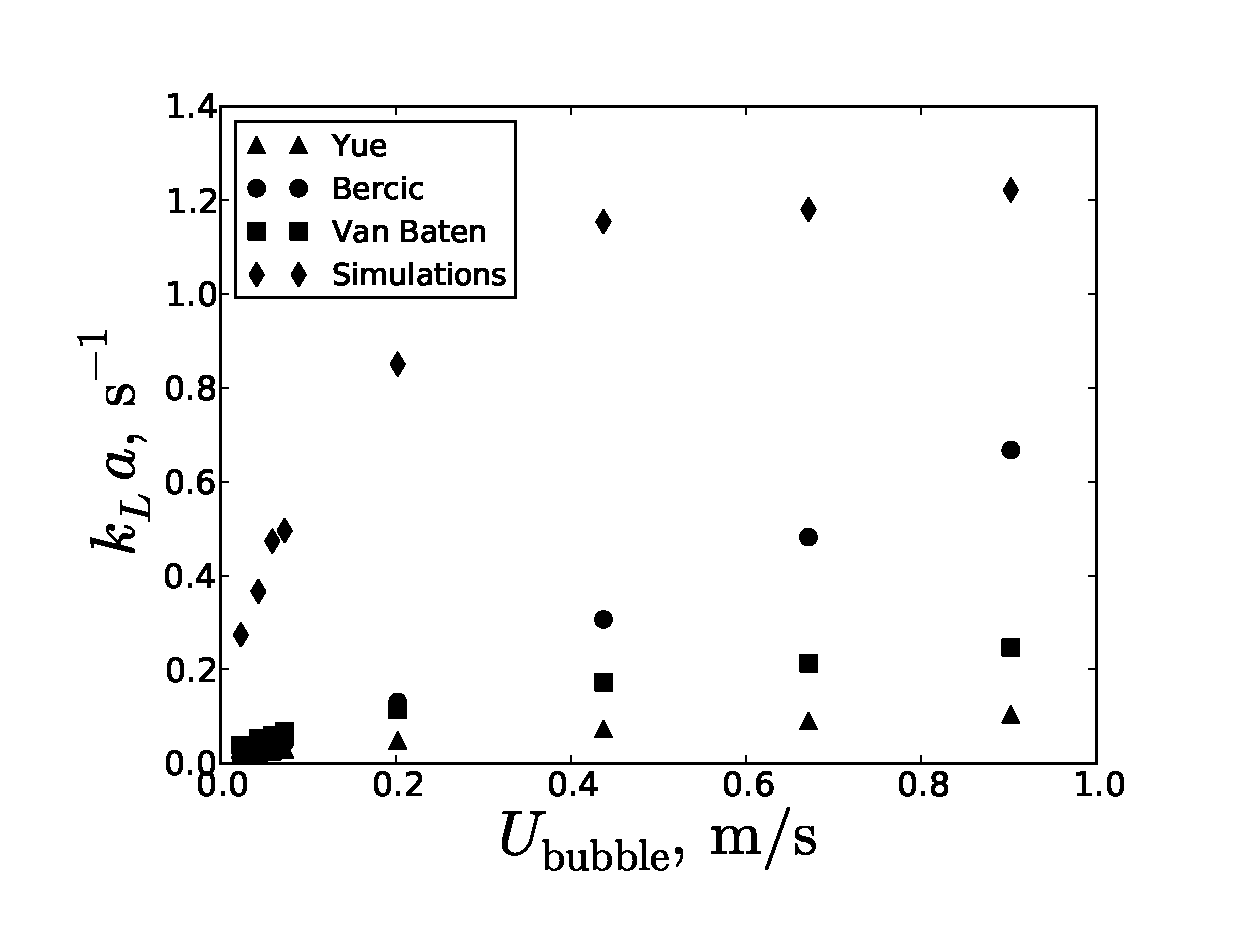
\includegraphics[width=\textwidth]{Figures/comparison_correlations.eps}
\caption{One can see the comparison between correlations and simulations. {\color{red} Last two
points can be eliminated due to improper imposement of the concave structure of the bubble. The
large deviation of the results can be probably explained by the flow between plates in comparison
with the flow in circular and square microchannels.} \label{fig:comparison:correlations}}
\end{figure}

\subsection{Average concentration}
As far as we used the inlet/outlet concentration in the expression of the calculation of the
volumetric mass transfer coefficient. However, the bubble in simulations located closely to the
inlet and with periodic boundary conditions that can change the volumetric mass transfer
coefficient significantly. As it will be discussed later in the appendix section, the assumption of
the periodic boundary conditions requires the continuous picture. The continuous picture requires as
well the average concentration to be of constant value. If the average concentration is used for
the calculation of the volumetric mass transfer coefficient {\color{red} (which can be more
adequate)}, then the volumetric mass transfer coefficient is more close to the correlation values,
see Fig. \ref{fig:average:concentration}. 
\begin{figure}[htb!]
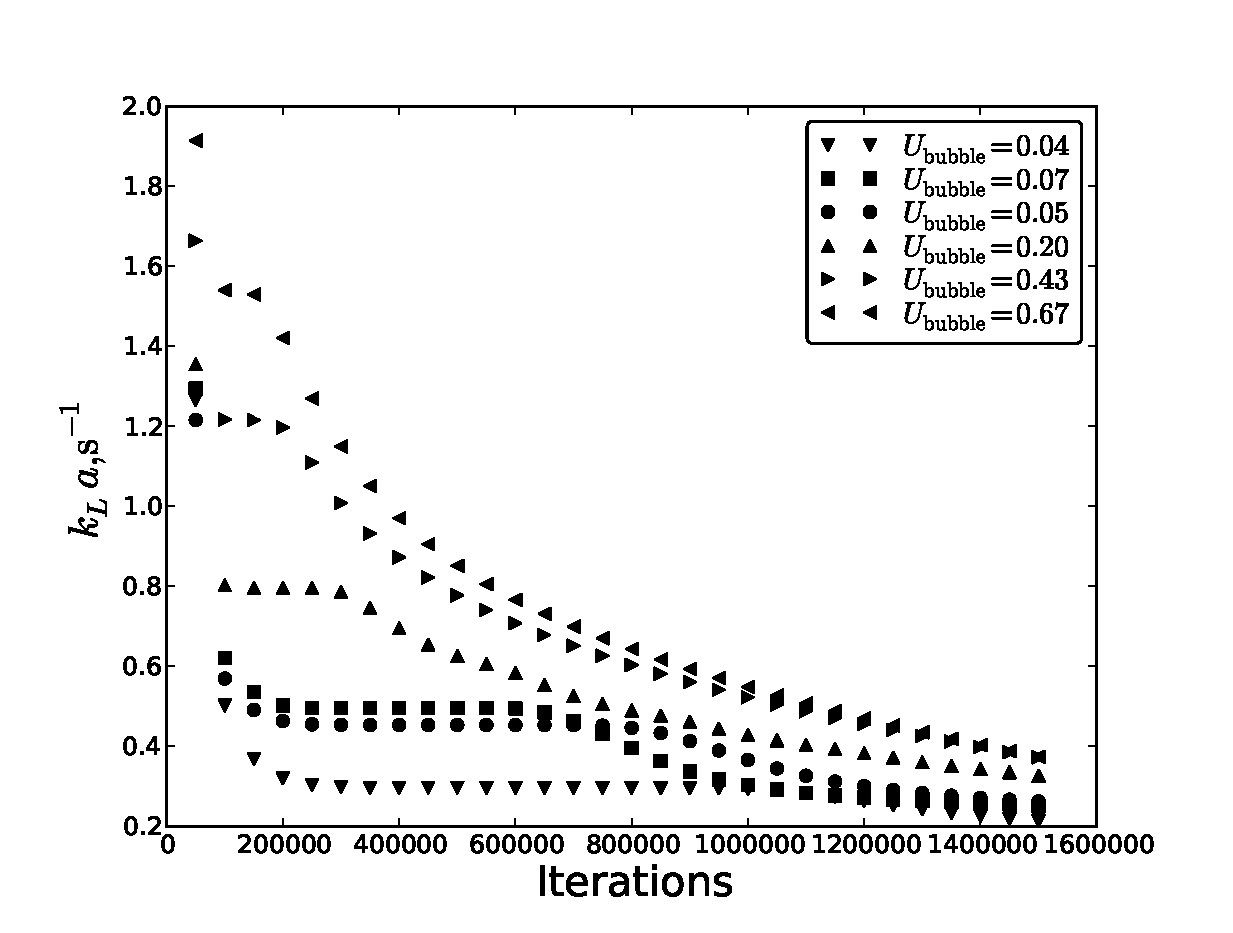
\includegraphics[width=\textwidth]{Figures/steady_state_average.eps}
\caption{The calculation of the volumetric mass transfer coefficient, if instead the inlet/outlet
concentration the average concentration is used.\label{fig:average:concentration}}
\end{figure}
One can see that the average concentration requires more than 2 millions time iterations to come to
the steady-state.

\section{Other boundary conditions}
We used the outflow boundary conditions for both boundaries and determined the coefficient
according Eq. \ref{theor:continuous:mass:transfer}. One can see the calculated mass transfer
coefficient in time in Fig. \ref{fig:steady:state:jos}.
\begin{figure}[htb!]
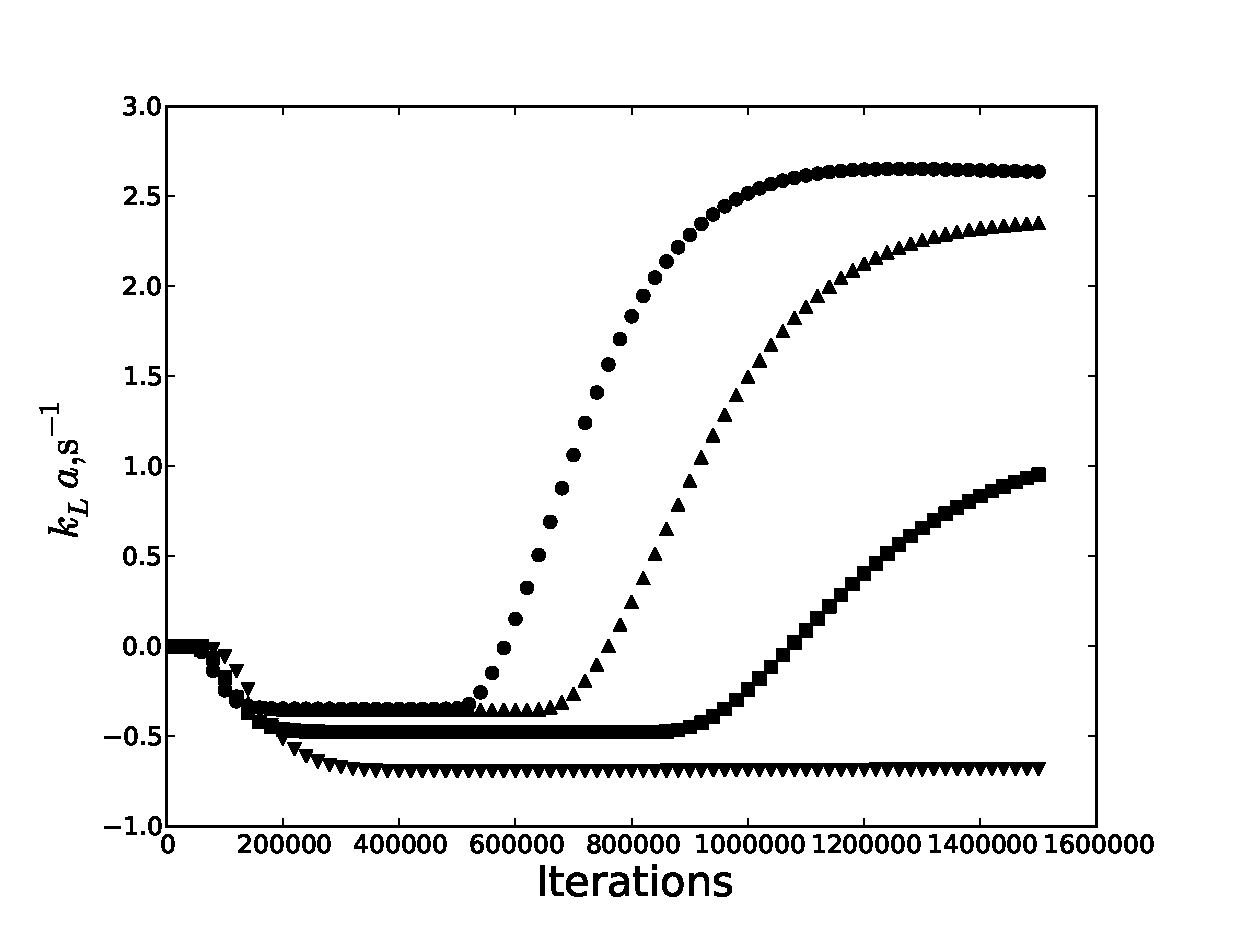
\includegraphics[width=\textwidth]{Figures/steady_state_jos.eps}
\caption{The calculated mass transfer coefficient in time with open boundaries $\partial_x
C_{inlet}=\partial_x C_{outlet}=0$. One can see some negative values for volumetric coefficients.
This situation corresponds to the case, then the inlet concentration is greater than the outlet
$C_{inlet}>C_{outlet}$. This corresponds to smaller capillary numbers due to vortex in front of the
bubble. It is the indication that one needs to take more time steps to wait until the outlet
concentration becomes larger than the inlet, which can take a relatively large time period to
wait. Large numbers of the volumetric mass transfer coefficients means the insuffient number of
the unit volumes simulated, as the large difference in the outlet and inlet numbers means the
deviation from the continuous picture. \label{fig:steady:state:jos} }
\end{figure}
If two domains are joined together then results are quite different. One can see them in Fig.
\ref{fig:steady:state:jos:double}.
\begin{figure}
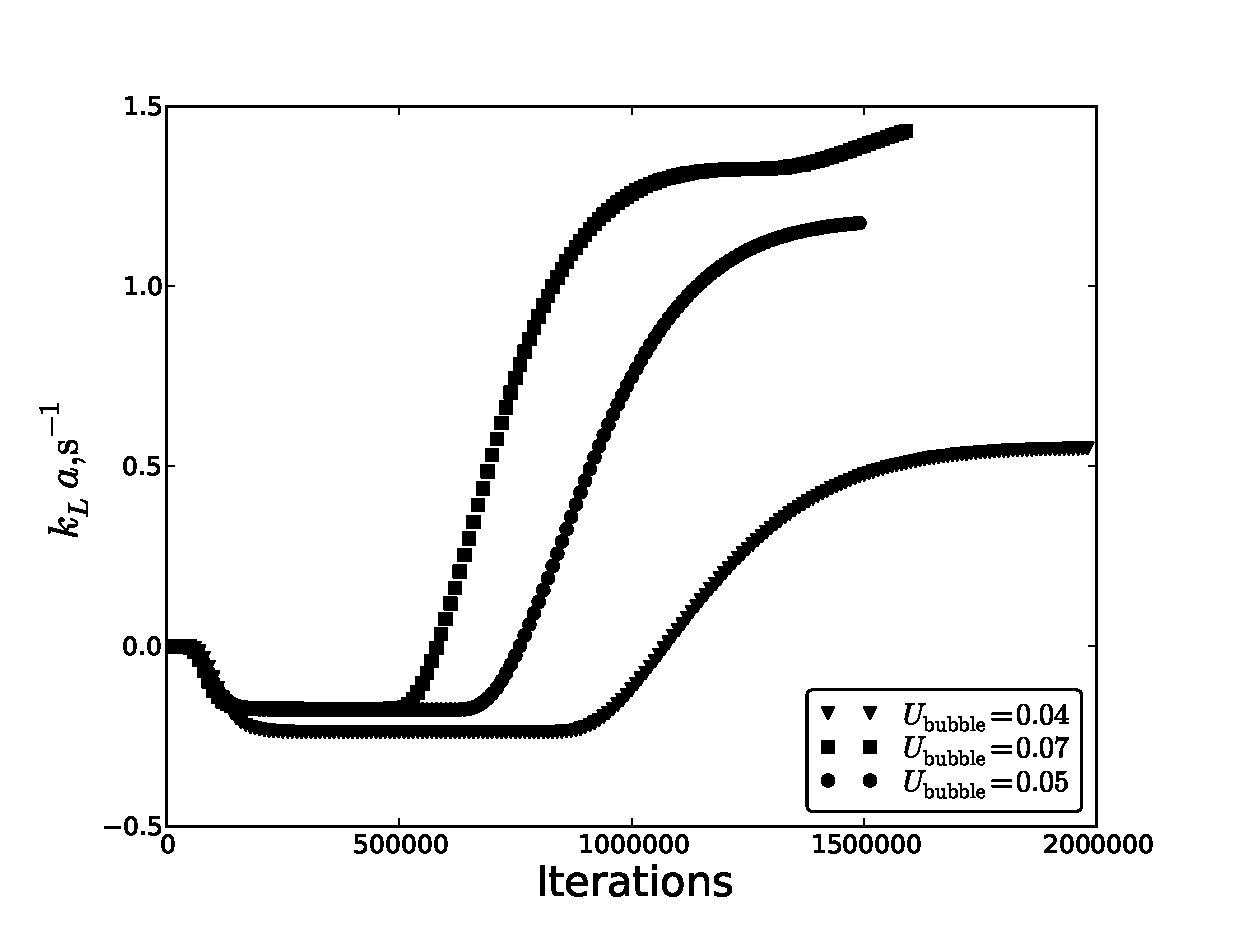
\includegraphics[width=\textwidth]{Figures/steady_state_double_jos.eps}
\caption{The mass transfer coefficient versus time for doubled domain. One can see that the
volumetric mass transfer coefficients are smaller in comparison with one unit volume simulation. As
well one needs to wait longer time as the mass comes from one bubble to another bubble. 
\label{fig:steady:state:jos:double}}
\end{figure}

\section{Grid Refinement}
We performed a grid refinement study and compared it with the original data. For this purpose we
doubled every fluid node and ran simulations. One can see {\color{red} That's what I have at the
moment - need to write parallel version for the grid refinement} in Fig. \ref{fig:grid:comparison}
the comparison between original size and refined grid simulations data. The results are close,
especially it's important for larger velocities, where diffusion layer is underresolved.
\begin{figure}[htb!]
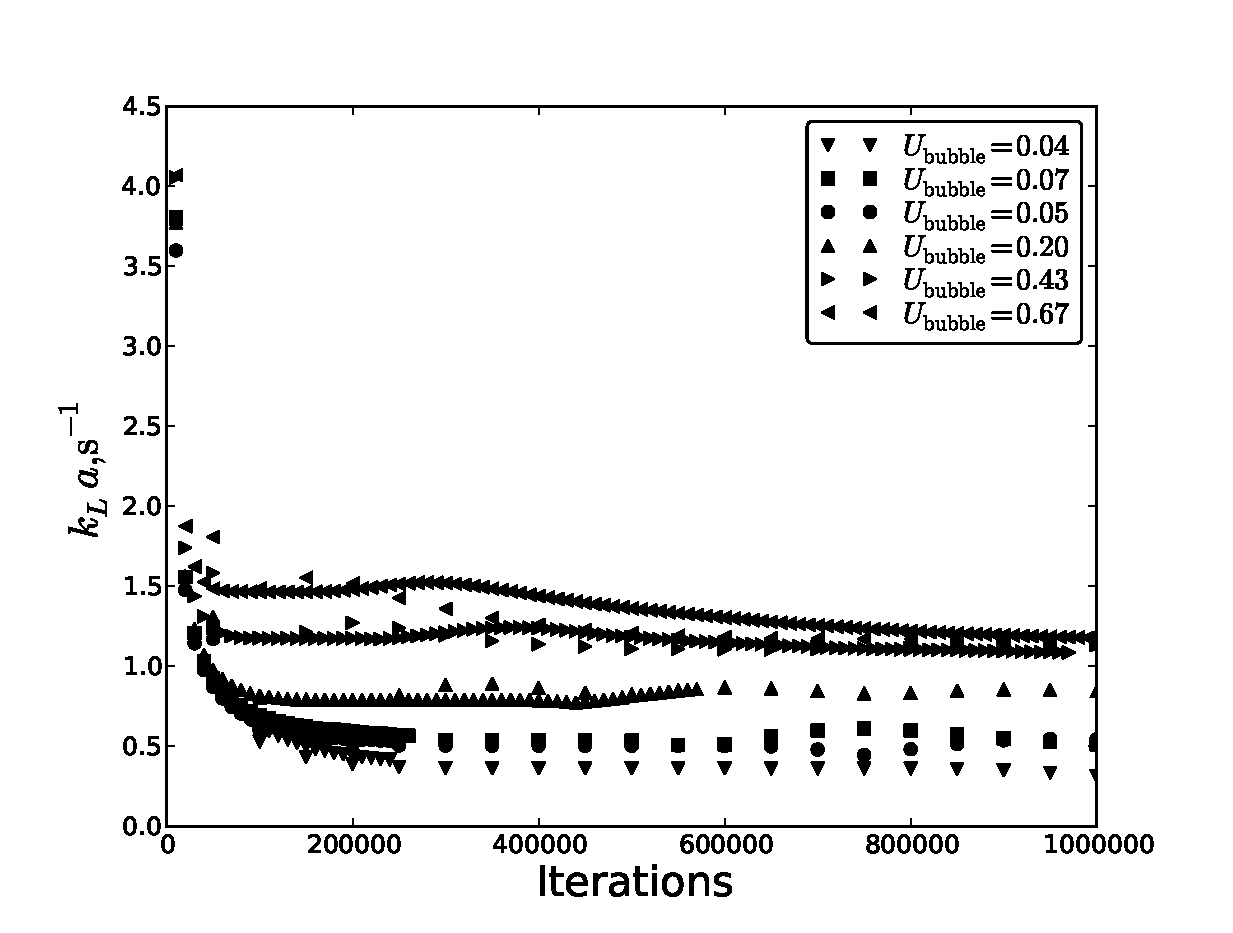
\includegraphics[width=\textwidth]{Figures/steady_state_comparison_grid.eps}
\caption{Comparison between the usual and refined grid simulations. One
can see that curves are close.\label{fig:grid:comparison}}
\end{figure}

\appendix

\section{Boundary conditions}
In what follows we will examine different LBM implementations:
\begin{description}
 \item[BB conditions] The walls can be treated via the simple bounce back rule:
\begin{equation}
f_{\bar{i}B}=f_{iF},\text{ for } \forall i,
\end{equation}
where $B$ is the boundary node with coordinates $\bm{r_F}+\bm{c_i}$, $F$ is the fluid node. This
will fulfill the macroscopic conditions as:
\begin{equation}
J_{fluid}= \sum_{c_i\cdot n>0}{f_i c_i}=J_{wall},
\end{equation}
which is in turn represents the following boundary condition:
\begin{equation}
\partial_n J_n=\partial_n C u_n = u_n \partial_n C=0
\end{equation}

The walls can be treated through simmetric boundary conditions as well, which are really close to
bounce-back formulation. In this case one can insure that the concentration values at the wall and
at the fluid equal to each other. 

For the constant concentration at the bubble surface one can use the pressure anti
bounce-back conditions
\cite{ginzburg-boundary-main}:
\begin{equation}
f_{iB}=-f^{*}_{iF}+2 e_i(W),
\end{equation}
where the subscript $*$ stands for after-collision population, $W$ stands for the wall
concentration to be imposed.
\item[Inamuro conditions] Inamuro boundary conditions impose strict conservation of the population
by utilizing diffuse interface kinetic boundary approach \cite{inamuro-scalar-boundary}. The
unknown populations $f_i=w_i \rho^{\prime}\text{ for } \bm{c_i}\cdot \bm{n}>0$ are prescribed
through the equilibrium conditions, where $\rho^{\prime}$ is an unknown parameter.Then the
prescribed wall condition is as: 
\begin{equation}
\rho^{\prime}=\frac{\rho_{w}-\sum_{i,\bm{c_i}\cdot\bm{n}\leq0}
f_i}{\sum_{i,\bm{c_i}\cdot\bm{n}>0}w_i}
\end{equation}
For the zero flux on the wall one can use another equation:
\begin{equation}
\rho^{\prime}=-\frac{i,\bm{c_i}\cdot\bm{n}\leq0}{\sum_{i,\bm{c_i}\cdot \bm{n}}{w_i \bm{c_i}\cdot
\bm{n}}}.
\end{equation}
\end{description}

\section{Mass transfer definitions}
By the definition the mass transfer coefficient is the following:
\beq
k_L=\frac{\dot{m}}{P \Delta C},
\feq
where $\dot{m}$ is the mass rate $\Bigl[\frac{kg}{s}\Bigr]$, $P$ is the area of the surface
$\Bigl[m^2\Bigr]$, $\Delta C$ is the concentration difference $\Bigl[\frac{kg}{m^3}\Bigr]$.
Therefore, $k_L$ has a dimension of velocity $\Bigl[\frac{m}{s}\Bigr]$. 

There are different methods to estimate the mass transfer coefficient $k_L$. We first examine the
theoretical definitions of the mass transfer in case of the point sources.
\subsection{Point mass sources}
In what follows we will present three approaches to calculate the mass points mass transfer
coefficients:
\begin{enumerate}
\item
Let us look at the infinitisemal small domain of the volume $A \Delta x$ in a steady-state, not
moving and with the mass source. Then the concentration difference can be found as $\Delta C = C^* -
C(t)$, where $C^*$ is the imposed concentration on the infinitesimal concentration source, $C(t)$ is
the time depending average concentration. Therefore one can write the time dependent ODE for the
average concentration in the domain:
\beq
\dot{m}= A \Delta x \frac{\mathrm{d}C}{\mathrm{d} t} = k_L P (C^{*}-C(t)), 
\feq
with the initial condition $C(0)=0$
The solution in time becomes as follows:
\beq
C(t)= C^{*}(1-\exp(-k_L a t )), 
\feq
where $k_L a$ is the volumetric mass transfer coefficient.

\item
The previous consideration is able to predict mass transfer happening in moving with the velocity
$U$ liquid, see Fig. \ref{fig:moving:frame}.
\begin{figure}[htb!]
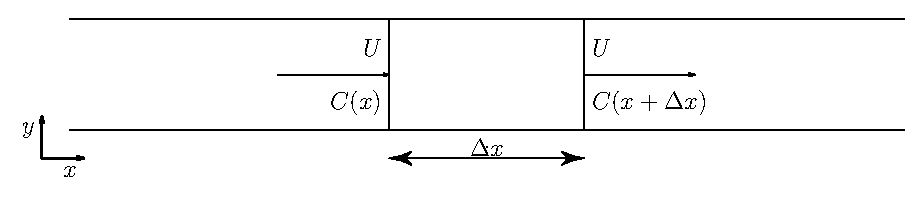
\includegraphics[width=\textwidth]{Figures/mass_transfer.eps}
\caption{The mass transfer in the moving liquid. \label{fig:moving:frame}}
\end{figure}

The mass accumulated in the unit volume $V=A \Delta x$ can be calculated as the difference of 
mass fluxes entering and leaving domain $U \bigl(C(x+\Delta x)-C(x)\bigr)$. We assume that the
source is a point source with the effective perimeter P. The accumulated mass should be proportional
to the mass transfer coefficient:
\beq
U \bigl(C(x+\Delta x)-C(x)\bigr)=k_L P \bigl(C^{*}-C(x)\bigr), 
\feq 
giving the same equation but only in the coordinate domain:
\beq
C(x)= C^{*}\Bigl(1-\exp\bigl(-k_L a \frac{x}{U} \bigr)\Bigr).
\label{main:mass:transfer:expression} 
\feq

\item If one transfers to the frame moving with the liquid velocity $U$, then the situation will be
the same as in the first case. However, one can connect the time and spatial location with the
velocity $U$ ($t=\frac{x}{U}$) to obtain the same equation as in the case 2.
\end{enumerate}

The expression (\ref{main:mass:transfer:expression}) was used in the experiments by
\citet{bercic-mass}. One should be accurate with the definition of velocities because we have two
different phases. Usually, one can take the velocity $U$ to be as
average velocity or $U=U_{gas}+U_{liq}$, where $U_{gas}$ and $U_{liq}$ are liquid and gas
superficial velocities correspondingly. In this case, the continuouty assumption is restored and
all considerations above are valid.

 However, if one wants to analytically estimate the mass transfer coefficients, the situation is
much more complicated because of the two phases presence. Phases can have different mixing patterns
from film to slug and from slug to film. The analytical approaches described above assume that the
contributions from film and bubble caps can be calculated separately. However one can see that such 
an assumption for bubble caps (slug well mixed and the concentration is uniformly distributed over
the slug) usually overpredicts the mass transfer \cite{irandoust}. This happens since some tracer
concentration from film is mixed with the slug and changes the overall concentration in the slug.
Another issue is that if the slug is long enough then the film saturates with the tracer
concentration and its influence on the mass transfer can be negligible \cite{vanbaten-circular}.
Mixing patterns of the film and the liquid slugs are of great importance for the analytical
estimation of the mass transfer \cite{yue-mass}.
 
\subsection{Numerical calculation}
In the numerical simulation it is not possible to simulate really long domains with the infinite
number of the bubbles. As we saw before there are two approaches towards it - either to simulate
the bubble train and then to measure concentration along the pipe, Eq.
\ref{main:mass:transfer:expression}, or to transfer to the reference frame moving with bulk
velocity $U$ and conduct the same measurements through Eq. \ref{main:mass:transfer:expression}.
However, both methods do require a tracking of moving bubbles which is complicated from the
numerical point of view.

Therefore, one needs to come up with the simple smaller domain calculations
of the mass transfer coefficient, which represent the continuous picture with infinite numbers of
the bubbles closely. In comparison with analytical estimations of the mass transfer coefficient,
where the mixing patterns are extremely important, the numerical simulations need only to mimic
the continous picture and provide the way to calculate the volumetric mass transfer coefficient. 

We perform simulations in the frame moving with the bubble (velocity
$U_{bubble}$), that the bubble position stands steady. The bubble velocity $U_{bubble}$ is
different from the bulk velocity $U_{gas}+U_{liq}$. In this case we need to perform coordinate
change:
\beqal
&x(t)=U_{bubble}t\\
&C(x)=C^{*}\Bigl(1-\exp\bigl(-k_L\, a \frac{x}{U_{gas}+U_{liq}}\bigr)\Bigr)\\
&C(t)=C^{*}\Bigl(1-\exp\bigl(-k_L\, a\, t \frac{U_{bubble}}{U_{gas}+U_{liq}}\bigr)\Bigr)
\feqal
If the unit volume that we simulate is quite long one can obtain the values of the concentration
in the inlet and outlet as a function of time:
\beqal
&C(U_{bubble}\, t)=C^{*}\Bigl(1-\exp\bigr(-k_L\, a\, t
\frac{U_{bubble}}{U_{gas}+U_{liq}}\bigr)\Bigr)\\
&C(U_{bubble}\,t+L_{unit})=C^{*}\Bigl(1-\exp\bigl(-k_L a \frac{
U_{bubble}\,t+L_{unit}}{U_{gas}+U_{liq}}\bigr)\Bigr)\\
&=C^{*}\Bigl(1-\exp\bigl(-k_L\, a\, t \frac{U_{bubble}}{U_{gas}+U_{liq}}\bigr)\exp\bigl(-k_L a
\frac{L_{unit}}{U_{gas}+U_{liq}}\bigr)\Bigr)
\feqal
Therefore the mass transfer coefficient can be calculated as follows:
\begin{equation}
\label{theor:continuous:mass:transfer}
\begin{aligned}
&-k_L a \frac{L_{unit}}{U_{gas}+U_{liq}}=\ln\Bigl(\frac{C^{*}-C_{outlet}}{C^{*}-C_{inlet}}\Bigr)\\
&k_L a
=\frac{U_{gas}+U_{liq}}{L_{unit}}\ln\Bigl(\frac{C^{*}-C_{inlet}}{C^{*}-C_{outlet}}
\Bigr)
\end{aligned}
\end{equation}
If inlet and outlet concentrations are small in comparison with the saturation concentration $C^{*}$
then the expression for the volumetric mass transfer coefficitent $k_L a$ can be simplified:
\beq
\vol=\frac{\Delta C}{C^{*}} \frac{U_{gas}+U_{liq}}{L_{unit}},
\feq
where $\Delta C=C_{outlet}-C_{inlet}$. If we go to the continuous formulation by changing $L_{unit}$
to be a continuous coordinate $x$, then the following can be obtained \cite{jos-mass}:
\beq
\Delta C = C^{*} \vol \frac{x}{U_{gas}+U_{liq}}
\label{small:conc:mass:estimation}
\feq

We consider the following possibilities of conducting numerical simulations:
\begin{enumerate}
 \item 
The tracer picking up procedure can be introduced
in the manner of the considerations above. We impose the concentration at the entrance to be
constant $C(0,y)=C_{inlet}$, at the outlet we impose the outflow boundary condition $\frac{\partial
C}{\partial x}(L,y)=0$. To be compliant with the considerations above one needs to impose as well
the outflow boundary conditions for the inlet as well. However, without loss of the generality one
can impose $C_{inlet}=0$, since the walls in the reference frame
moving with the bubble are moving from the inlet to the outlet. That means that no tracer
concentration leaves domain from the inlet side, which is true for the capillary numbers larger
than $0.6$.  However, this boundary condition can not be used in the case of small capillary
numbers, since there is a strong circulation in front of the bubble. One can see the sketch of the
approach in Fig. \ref{fig:benchmark:jos}. The longer the numerical domain length the better will be
results. One can estimate the volumetric mass transfer coefficient in this case through the equation
(\ref{small:conc:mass:estimation}) for small concentrations. Note a few considerations:
\begin{itemize}
\item  The considerations above were established for the homogenous velocity field. In the case of
the non-homogenous velocity field one needs to obtain a concentration from the mass flux:
\beq
C_{outlet}=\frac{\int{U(y) C(L_{unit},y) \mathrm{d}y}}{\int{U(y) \mathrm{d}y}}.
\feq
\item Note, that one cannnot use the definition of the mass transfer coefficient as far as it
varies through the bubble due to inhomogenoities of the flow. Therefore, the volumetric mass
transfer coefficient is introduced that takes into the account the bubble geometry.
\end{itemize}
\begin{figure}
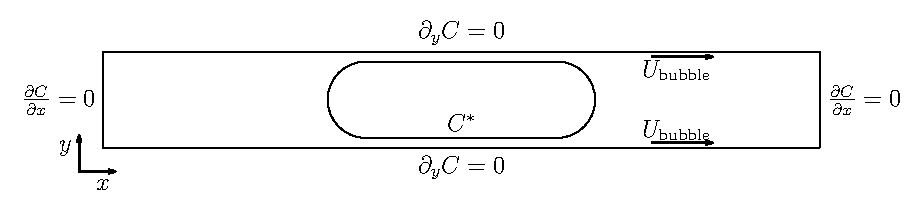
\includegraphics[width=\textwidth]{Figures/benchmark_jos.eps}
\caption{The numerical mass transfer benchmark. \label{fig:benchmark:jos}}
\end{figure}

\item Another possibility is to use the periodic boundary conditions as the limiting case of the
continuous formulation. In this case the inlet and outlet concentrations are not much different
($C(x)=C(x+L_{unit})=C(x+\Delta x)\approx C_{media}$, see Fig. \ref{fig:moving:frame}), where
$C_{media}$ is the mass averaged over domain concentration. This formulation requires the periodic
boundary condition $C_{inlet}=C_{outlet}$. By the definition the mass transfer coefficient is
proportional to the gain of the mass in the system divided by the concentration difference:
\beq
j=\frac{\dot{m}}{P \Delta C}=\frac{\dot{m}}{P (C^{*}-C_{media})},
\feq
where mass difference in the domain can be calculated as:
\beq
\dot{m}=\frac{m_2-m_1}{t_2-t_1}=\frac{\int_{C(t_2)\mathrm{d}V}-\int{C(t_1)\mathrm{d}V}}{t_2-t_1}.
\feq
Therefore the assumptions  of this approach is that the difference between inlet and outlet is not
considerably large and the tracer is well mixed in the slug, as one can take the concentration
difference as $\Delta C = C^{*}-C_{media}$. The best case scenario is when $C_{media}$ is close to
zero, in this case we can be sure that the flux to the domain is calculated precisely and periodic
boundary conditions are fulfilled.
\end{enumerate}
 

\section{Solution of the semi-infinite concentration problems}
\label{mass:transfer:correlation}
For short contact times the mass transfer can be decomposed into two parts: transfer from the wall
to semi-infinite medium and transfer from the sphere to the infinite medium. In what follows we
derive analytical solutions to these two situations:
\begin{description}
\item[Wall mass transfer] The problem by mathematically is stated as:
\begin{equation}
\begin{aligned}
&\partial_t C =D \partial^2_{xx} C\\
&C(x,0)=0\\
&C(0,t)=C_0\\
\end{aligned}
\end{equation}
As far as the problem is non-homogenious one needs to decompose the problem into the steady-state
and homogenous transient problem:
\begin{equation}
C=C_h + C_s,
\end{equation}
where $C_h$ and $C_s$ satisfy the following equations:
\begin{equation}
\begin{aligned}
&\frac{\mathrm{d^2} C_s}{\mathrm{d}x^2}=0 && \partial_t C_h=D\partial^2_{xx} C_h\\
&C_s(0)=C_0 && C_h(x,0)=-C_0\\
&C_s(\infty)=C_0 && C_h(0,t)=0\\
\end{aligned}
\end{equation}
One can easily check that the solution and boundary conditions are satisfied. The solution of
the steady-state problem is $C_s=C_0$. To find a solution of the semi-infinite medium we will use
the method of separation of variables:
\begin{equation}
\begin{aligned}
&C_h=\Theta(t)\Phi(x)\\
&\frac{1}{\Theta(t)}\frac{\mathrm{d}\Theta(t)}{\mathrm{d}t}=D
\frac{1}{\Phi(x)}\frac{\mathrm{d}^2\Phi(x)}{\mathrm{d}x}=-\alpha^2 D\\
\end{aligned}
\end{equation}
The solution for the time-dependent part is as:
\begin{equation}
\Theta(t)=\exp(-\alpha^2 D t).
\end{equation}
The solution for the spatial dependence function is as:
\begin{equation}
\Phi(x)=A\cos(\alpha x)+ B\sin(\alpha x).
\end{equation}
The overall solution of the homogenious part is represented as:
\begin{equation}
C_h=(A\cos(\alpha x) + B\sin(\alpha x)) \exp(-\alpha^2 D t),
\end{equation}
where one needs to solve the eigenvalue problem to find the necessary $\alpha$ parameter. One can
find it through the initial and boundary conditions:
\begin{equation}
\begin{aligned}
&C_h(x,0)=-C_0\\
&C_h(x,0)=A\cos(\alpha x)+B\sin(\alpha x)=-C_0\\
&C_h(0,t)=0\\
&C_h(0,t)=A\exp(-\alpha^2 D t)=0\\
&A=0\\
\end{aligned}
\end{equation}
Therefore one needs to decompose the constant $-C_0$ through the function $\sin(\alpha x)$. It can
be done through a continuous Fourier transform:
\begin{equation}
\begin{aligned}
&C_h=\int_{\alpha>0}{B(\alpha) \sin(\alpha x) \exp(-\alpha^2 D t) \mathrm{d}\alpha}\\
&C_h(x,0)=-C_0=\int_{\alpha>0}{B(\alpha)\sin(\alpha x) \mathrm{d}\alpha}\\
&\int_{0}^{\infty}{B(\alpha) \frac{e^{i\alpha x}-e^{-i\alpha x}}{2 i}\mathrm{d} \alpha}=-C_0\\
\end{aligned}
\end{equation}
To get function $B(\alpha)$ one needs to proof the following Fourier relationship:
\begin{equation}
\begin{aligned}
&F(x)=\frac{2}{\pi}\int_{\alpha=0}^{\infty}{\mathrm{d}\alpha \sin(\alpha x)
\int_{x'=0}^{\infty}{\sin(\alpha x')F(x')\mathrm{d} x'}}\\
&\frac{2}{\pi}\int_{\alpha=0}^{\infty}{\mathrm{d}\alpha \sin(\alpha x)\sin(\alpha x')}=\frac{2}{\pi}
\int_{\alpha=0}^{\infty}{\mathrm{d}\alpha \frac{\cos(\alpha(x+x'))-\cos(\alpha(x-x'))}{2}}\\
&=\frac{1}{\pi}\int_{\alpha=0}^{\infty}{\mathrm{d}\alpha\Bigl[\frac{e^{i\alpha
(x+x')}+e^{-i\alpha(x+x')}}{2}-\frac{e^{i\alpha
(x-x')}+e^{-i\alpha(x-x')}}{2}\Bigr]}\\
&=\frac{1}{2\pi}\int_{\alpha=-\infty}^{\infty}{\mathrm{d}\alpha\Bigl[e^{i\alpha(x+x')}-e^{
i\alpha(x-x')} \Bigr]}=\delta(x+x')-\delta(x-x')\\
&F(x)=\int_{x'=0}^{\infty}{\mathrm{d} x' (\delta(x+x')-\delta(x-x')) F(x')}=F(x) 
\end{aligned}
\end{equation}
Therefore the solution is as follows:
\begin{equation}
C_h(x,t)=-\frac{2 C_0}{\pi}\int_{\alpha>0} {\exp{-\alpha^2 t} \int_{x'>0}{\sin(\alpha x) \sin(\alpha
x')}} 
\end{equation}
Integrals can be taken from \citet{ozisik}:
\begin{equation}
\begin{aligned}
&\frac{2}{\pi}\int_{\alpha=0}^{\infty}{e^{-\alpha^2 D t} \sin(\alpha x) \sin(\alpha
x')}\\
&=\frac{1}{\sqrt{4\pi D t}}\biggl[\exp\Bigl(-\frac{(x-x')^2}{4 D
t}\Bigr)-\exp\Bigl(-\frac{(x+x')^2}{4 D t}\Bigr)\biggr]
\end{aligned}
\end{equation}
The final answer for homogenous part becomes \cite{ozisik}:
\begin{equation}
C_h(x,t)=-C_0\mathrm{erf}\Bigl(\frac{x}{\sqrt{4 D t}}\Bigr),
\end{equation}
where $\mathrm{erf}$ stands for the error function defined as:
\begin{equation}
\mathrm{erf(y)}=\frac{2}{\sqrt{\pi}}\int_{0}^{y}{e^{-\eta^2}\mathrm{d}\eta}.
\end{equation}
Overall solution then is defined as:
\begin{equation}
C(x,t)=C_0-C_0\mathrm{erf}\Bigl(\frac{x}{\sqrt{4 D t}}\Bigr),
\end{equation}
with the mass transfer coefficient is defined as the integral of absorbed gas upto time $t_e$
divided by the time $t_e$. The accumulated  flux is the integral of the derivative
$-D\frac{\mathrm{d} C(x,t)}{\mathrm{d}x}|_{x=0}$ by time $t$. The incoming flux is as follows:
\begin{equation}
\begin{aligned}
&-D\frac{\mathrm{d} C(x,t)}{\mathrm{d}x}|_{x=0}=D \frac{1}{\sqrt{\pi D t}}\\
\end{aligned}
\end{equation}
The accumulated concentration and the mass transfer coefficients are:
\begin{equation}
\begin{aligned}
&\int_{0}^{t_{\mathrm{film}}}{-D\frac{\mathrm{d} C(x,t)}{\mathrm{d}x}|_{x=0} \mathrm{d}t}=2
\sqrt{ \frac{D t}{\pi}}\\
&k_L = 2 \sqrt{\frac{D}{\pi t_{\mathrm{film}}}}.
\end{aligned}
\end{equation}
If we account for the two surfaces for the bubble then one can obtain the following volumetric mass
transfer coefficient:
\begin{equation}
\begin{aligned}
&k_L a= 2\sqrt{\frac{D}{\pi t_{\mathrm{film}}}} 2
\frac{L_{\mathrm{bubble}}-(H_{\mathrm{eff}}-2\delta)}{(L_{\mathrm{bubble}}+L_{
\mathrm { slug } } )H_ { \mathrm { eff } } }\\
&k_L a= 2\sqrt{\frac{D}{\pi
\frac{L_{\mathrm{bubble}}-(H_{\mathrm{eff}}-2\delta)}{U_{\mathrm{bubble}}}}} 2
\frac{L_{\mathrm{bubble}}-(H_{\mathrm{eff}}-2\delta)}{(L_{\mathrm{bubble}}+L_{
\mathrm { slug } } )H_ { \mathrm { eff } } }\\
&k_L a=4 \sqrt{\frac{D U_{\mathrm{bubble}}}{\pi}}
\frac{\sqrt{L_{\mathrm{bubble}}-(H_{\mathrm{eff}-2\delta})}}{(L_{\mathrm{bubble}}+L_{\mathrm{slug}}
)H_ { \mathrm { eff } } }
\end{aligned}
\end{equation}

\item[Cylinder mass transfer] For the cylinder mass transfer one needs to solve the heat conduction
equation one needs to use cylindrical coordinates. The system is prescribed by the following set
of equations:
\begin{equation}
\begin{aligned}
&\frac{\partial C}{\partial t}=D\frac{\partial^2 C}{\partial r^2} + \frac{D}{r}\frac{\partial
C}{\partial r}\\
&C(a,t)=0\\
&C(r,0)=0\\
\end{aligned}
\end{equation}
The solution is given by \citet{ozisik} as:
\begin{equation}
\begin{aligned}
&C(r,t)=C_0\\
& - C_0\int_{\alpha=0}^{\infty}{\mathrm{d}\alpha \frac{\alpha}{J_0^2(\alpha
a)+Y_0^2(\alpha a)}e^{-\alpha^2 D t}[J_0(\alpha r) Y_0(\alpha a)-Y_0(\alpha r) J_0(\alpha a)]}\\
&\times \int_{r'=a}^{\infty}{r'[J_0(\alpha r')Y_0(\alpha a)-Y_0(\alpha r') J_0(\alpha
a)]\mathrm{d}r'}
\end{aligned}
\end{equation}
These integrals can be taken through the recurrent equations for Bessel functions. However, the
penetration of the concentrator comes not only from the diffusion but mainly from the advection
part. According to the penetration theory one can use the following correlation for the mass
transfer coefficient:
\begin{equation}
k_L=2\sqrt{\frac{D}{\pi t_{\mathrm{contact}}}},
\end{equation}
where $t_{\mathrm{contact}}$ for the bubble cap can be calculated from the following considerations
\cite{vanbaten-circular}: the distance travelled by a fluid packet coming to the bubble equals to a
half of semicircle perimeter until it is swept away by the vortex in the front of the bubble
{\color{red} (working only for small capillary numbers where a vortex exists in the front of the
bubble)}. Therefore for the case of the bubble arising with the velocity $U_{\mathrm{bubble}}$ one
can estimate the mass transfer coefficient as follows:
\begin{equation}
k_L=2\sqrt{\frac{D}{\pi t_{\mathrm{contact}}}}=2\sqrt{\frac{D}{\pi \frac{ \pi
(H_{\mathrm{eff}}-2\delta)/2}{U_{\mathrm{bubble}}}}}=\frac{2\sqrt{2}}{\pi}\sqrt{\frac{D
U_{\mathrm{bubble}}}{H_{\mathrm{eff}}-2\delta}}
\end{equation}
The volumetric mass transfer coefficient is then as follows:
\begin{equation}
\begin{aligned}
k_L a=\frac{2\sqrt{2}}{\pi}\sqrt{\frac{D
U_{\mathrm{bubble}}}{H_{\mathrm{eff}}-2\delta}} \frac{\pi
(H_{\mathrm{eff}}-2\delta)}{(L_{\mathrm{bubble}}+L_{\mathrm{slug}}) H_{\mathrm{eff}}}\\
k_L a=2\sqrt{2}\sqrt{D
U_{\mathrm{bubble}}}\frac{\sqrt{H_{\mathrm{eff}}-2\delta}}{(L_{\mathrm{bubble}}+L_{\mathrm{slug}})H_
{\mathrm{eff}}}
\end{aligned}
\end{equation}

\end{description}
Therefore the overall adjusted for the flow between plates mass transfer coefficient is expressed as
follows:
\begin{equation}
\begin{aligned}
k_L a =&4 \sqrt{\frac{D U_{\mathrm{bubble}}}{\pi}}
\frac{\sqrt{L_{\mathrm{bubble}}-(H_{\mathrm{eff}-2\delta})}}{(L_{\mathrm{bubble}}+L_{\mathrm{slug}}
)H_ { \mathrm { eff } } }\\
&+2\sqrt{2}\sqrt{D
U_{\mathrm{bubble}}}\frac{\sqrt{H_{\mathrm{eff}}-2\delta}}{(L_{\mathrm{bubble}}+L_{\mathrm{slug}})H_
{\mathrm{eff}}}.
\end{aligned}
\end{equation}
 

\section{TRT $D2Q9$ model. Equilibrium functions}
One of the advantages of $D2Q9$ TRT model in comparison with $D2Q5$ usually used for simulations of
the advection-diffusion model is that $D2Q9$ is able to reduce numerical diffusion from diagonal
and non-diagonal diffusion tensor components \cite{kuzmin-stability-optimal}.

In
comparison with the BGK collision operator the TRT collision operator \cite{ginzburg-boundary-main}
decomposes the populations and the equilibrium
distribution into the symmetric and antisymmetric parts:
\begin{equation}
\label{trtdecomp}
f^{\pm}_i=\frac{f_i\pm f_{\bar{i}}}{2}\;,\; 
{eq_i}^{\pm}=\frac{eq_i\pm eq_{\bar{i}}}{2}\;,
\end{equation}
where $\bar{i}$ is the opposite direction to the $i$-th direction.
The collision is performed with two independent relaxation rates for 
symmetric and antisymmetric modes:
\begin{equation}
\label{trt}
\begin{aligned}
&f_i^{*}(\bm{x},t)=f_i(\bm{x},t)-\omega_{+} (f_i^{+} - eq_i^+)-\omega_{-}
(f_i^{-} -
eq_i^-)\\
&f_i(\bm{x}+\bm{c_i},t+1)=f_i^{*}(\bm{x},t).
\end{aligned}
\end{equation}
Note that the BGK collision operator is the particular subclass of the TRT relaxation operator with
$\omega_{+}=\omega_{-}$. In comparison with the BGK collision operator,
the TRT collision operator has the additional degree of freedom. Thus, the TRT operator then
introduces
so-called magic (free) parameter
$\Lambda=\Bigl(\frac{1}{\omega_{+}}-\frac{1}{2}\Bigr)\Bigl(\frac{1}{\omega_{-}}-\frac{1}{2}\Bigr)$. 
This free parameter controls the effective location of the bounce-back
walls \cite{ginzburg-multireflection}, second-order accuracy of
boundary \cite{ginzburg-boundary-main} and interface schemes \cite{ginzburg-discontinious}, 
spatial accuracy \cite{ginzburg-recurrence,servan-trt-stability},
consistency \cite{ginzburg-brinkman} and, to some extent,
stability \cite{kuzmin-stability-optimal,kuzmin-d1q3,servan-trt-stability}.
In particular, $\Lambda=\frac{1}{4}$ achieves the optimal stability for the
linear advection-diffusion isotropic equation \cite{kuzmin-stability-optimal}. 

The equilibrium functions for $D2Q9$ TRT model are represented as \cite{kuzmin-stability-optimal}:
\begin{equation}
\begin{aligned}
&eq_i^{+}=eq_i^{(m)}+g^{(u)} eq_i^{(u)}\\
&eq_i^{(m)}=t_i^{(m)} c_e+ eq_i^{(a)}\\
&eq_i^{(u)}=t_i^{(u)} \frac{u_x^2+u_y^2}{2}+\frac{u_x^2-u_y^2}{4} p_i^{(xx)}+g_{xy}^{(u)}\frac{u_x
u_y}{4} p_i^{xy}\\
&eq_i^{(a)}=\frac{D_{xx}-D_{yy}}{4} p_i^{xx}+\frac{D_{xy}}{4} p_i^{(xy)},
\end{aligned}
\end{equation}
where $p_i^{(xx)}=c_{ix}^2-c_{iy}^2$ and $p_i^{(xy)}=c_{ix} c_{iy}$. 

The following equilibrium functions solve the anisotropic advection-diffusion equation with the
following diffusion tensor:
\begin{equation}
D=
\begin{pmatrix}
D_{xx} + (g^{(u)}-1) u_x^2 & D_{xy}+(g_{xy}^{(u)}-1)u_x u_y\\
D_{xy} + (g_{xy}^{(u)}-1) u_x u_y& D_{yy}+(g^{(u)}-1) u_y^2 
\end{pmatrix}
\end{equation}
To consider the situation when the resolution is not needed to be changed in $x$ and $y$
directions, one can obtain that $D_{xx}=D_{yy}$. The cross-diagonal components of the diffusion
tensor are taken as zeros, i.e. $D_{xy}=0$. The numerical diffusion can be avoided by proper choice
of the equilibrium functions, i.e. $g_{xy}^{(u)}=g^{(u)}=1$.

As far as the simulated diffusion tensor is close to $0$ the stability limits restrict the velocity
amplitude to be simulated \cite{kuzmin-stability-optimal}. However, particular choice of weights
can drastically help. Fig. \ref{stability:d2q9} shows the stability limits for D2Q9 with removed
numerical diffusion and with it for two particular choices of weights.
\begin{figure}[htb!]
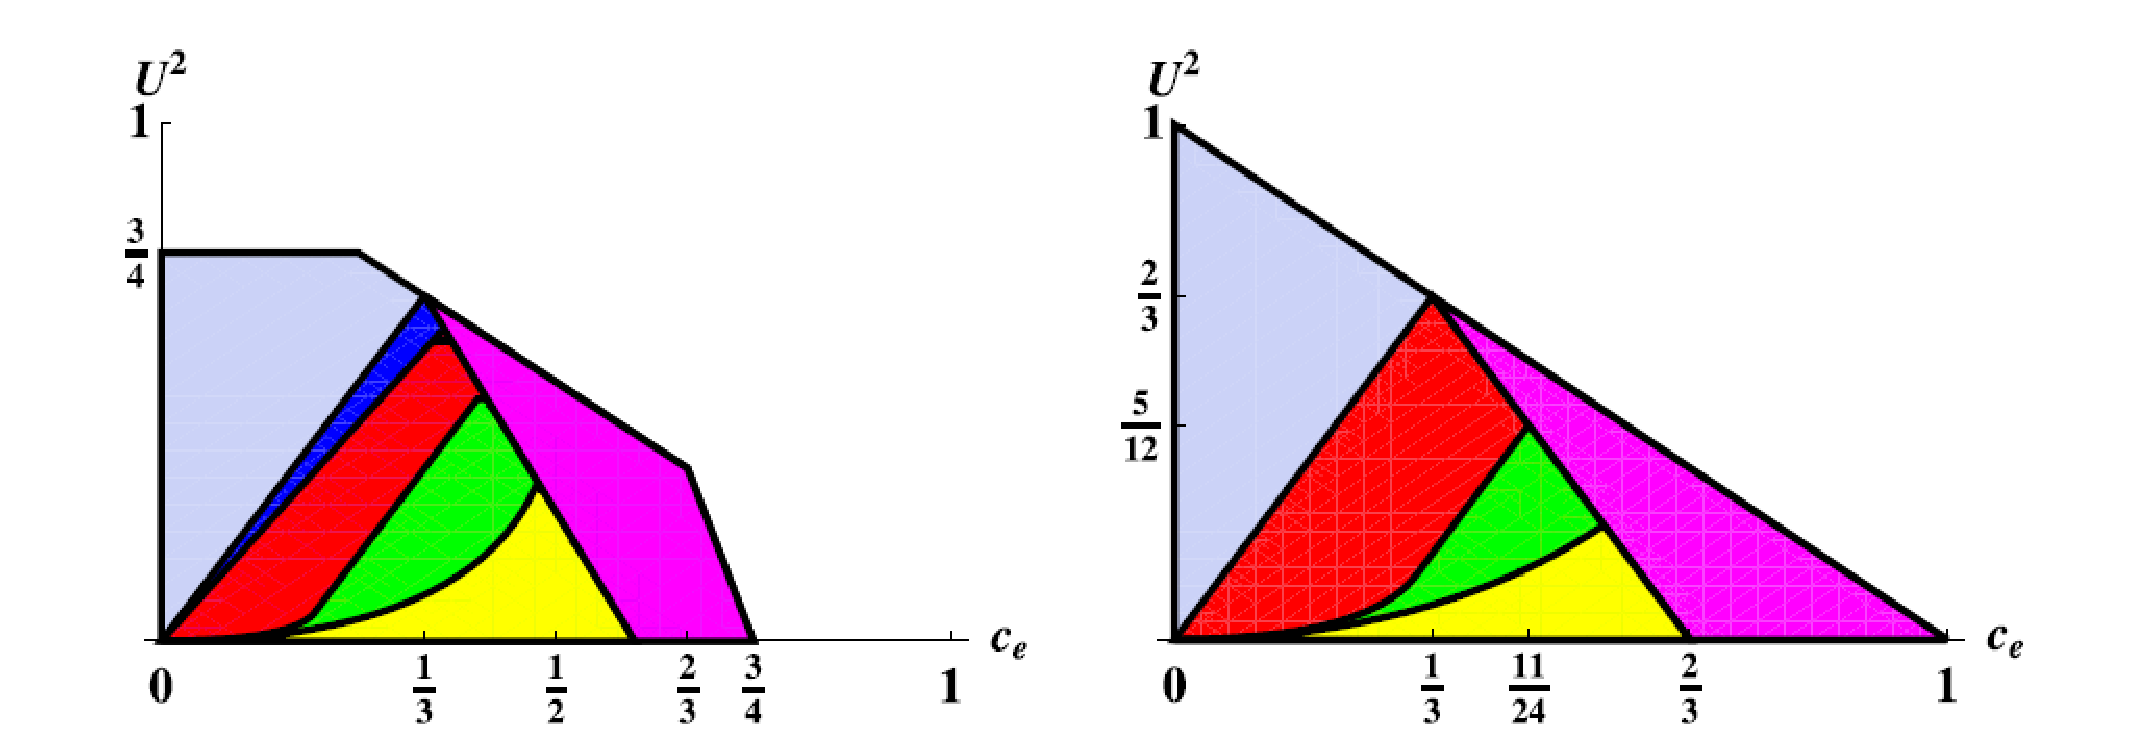
\includegraphics[width=\textwidth]{Figures/d2q9_stability.eps}
\caption{The non-negativity areas and stable sub-domains of the OTRT schemes ($\Lambda=\frac{1}{4}$)
are plotted for the $D2Q9$ (standard weights, left) and the $D2Q9$ (uniform weights, right) when the
numerical diffusion is removed, partially or completely. Two non-negativity areas where all the
equilibrium populations are positive have curvilinear boundaries: they are smaller when
$g^{(u)}_{xy}=0$ (yellow) and than when $g^{(u)}_{xy}=1$ (green+yellow). The non-negativity
condition is required by BGK collision operator. The stable sub-domains for $g^{(u)} = 1,
g^{(u)}_{xy} = 0$ are small (red+green+yellow) triangles. When the numerical diffusion is removed
the stable area is bounded by magenta and the (blue) domain above. The proper choice of weights can
allow to obtain  total triangle $0 \leq u_x^2+u_y^2 \leq 1−c_e$ (the
uniform weights only).
\label{stability:d2q9}}
\end{figure}

From here on we will use the standard weights as:
\begin{equation}
t_i^{(u)}=t_i^{(m)}=t_i^{(a)}=\Bigl\{0,\frac{1}{3},\frac{1}{3},\frac{1}{3},\frac{1}{3},\frac{1}{12},
\frac {1}{12},\frac{1}{12},\frac{1}{12}\Bigr\}
\end{equation}

\bibliographystyle{unsrtnat}
\bibliography{paper}

\end{document}
